\chapter{Chapter 8: Embedded Code Development \& Prototype to Reality}

This chapter compiles lecture-quality study notes and comprehensive exam answers for \textbf{Unit VIII: Embedded Code Development \& Prototype to Reality} of the OE-EC803A syllabus, adhering strictly to the \textbf{MAKAUT Answer Writing Guidelines}.


\section{Section 1: Writing Embedded Code for Resource-Constrained IoT Devices (Q8.1) [5M]}

\subsection{1. Introduction}
IoT edge devices are built around resource-constrained microcontrollers with severely limited RAM (often 2–256 KB), flash storage (32 KB–1 MB), and battery capacity. Writing embedded firmware for these platforms demands rigorous attention to \textbf{memory management}, \textbf{power optimization}, and \textbf{library selection}.

\begin{figure}[H]
\centering
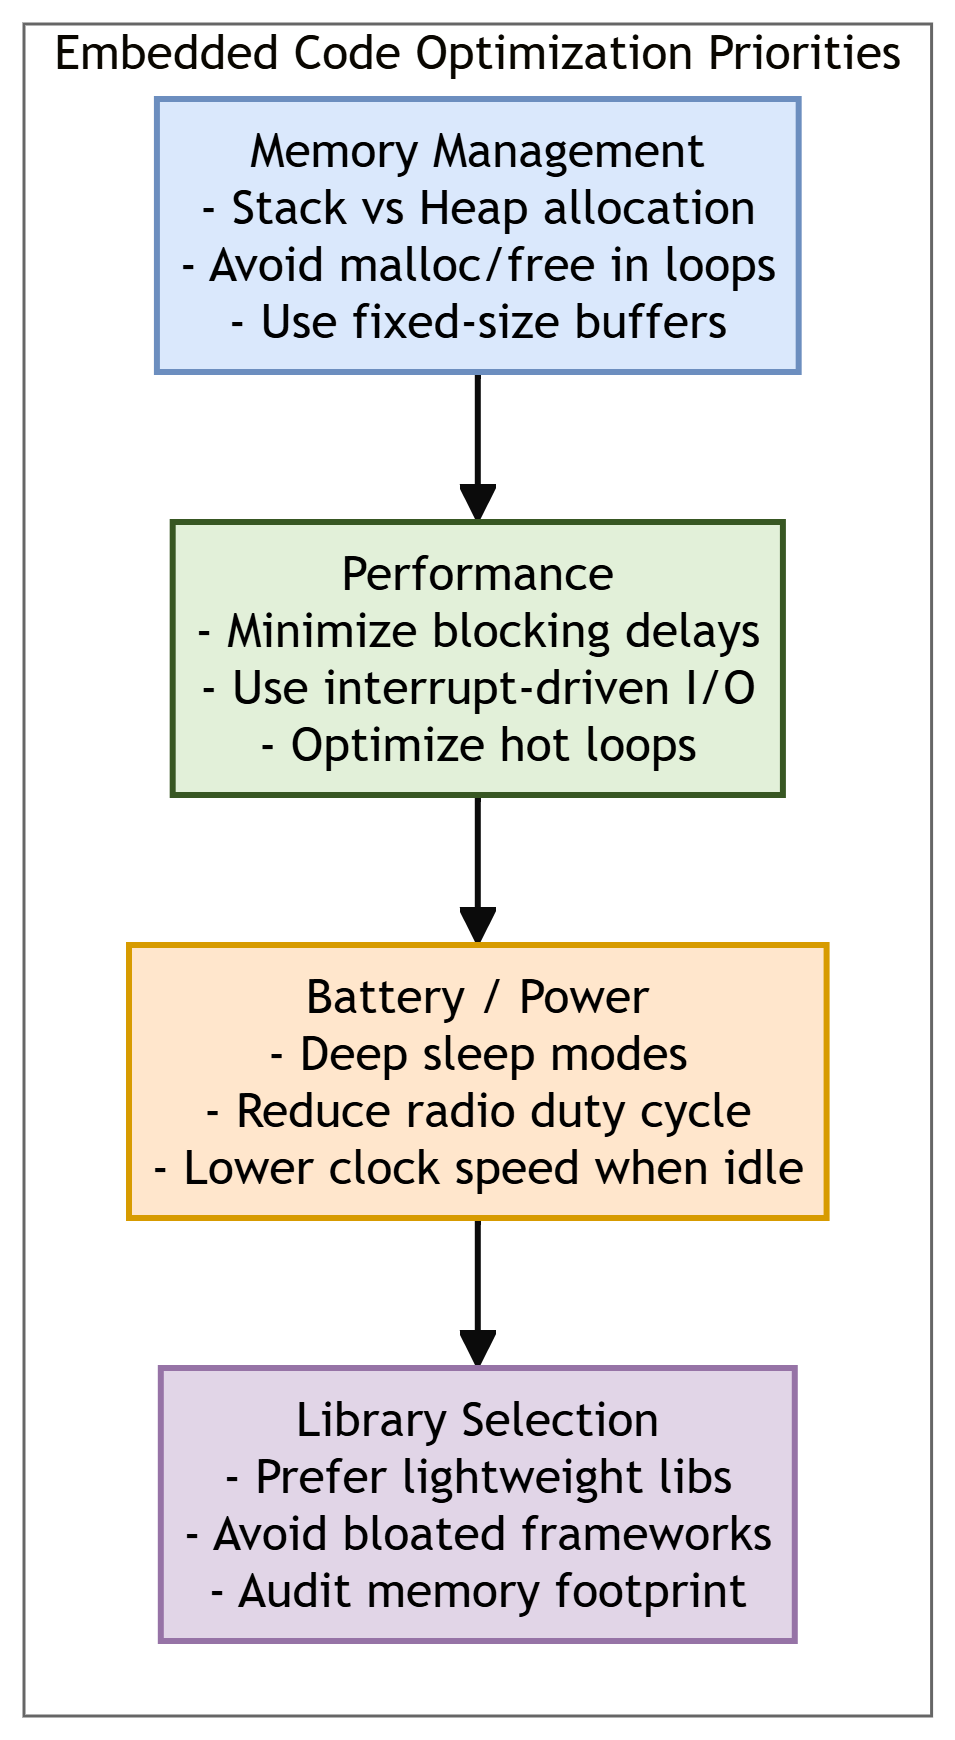
\includegraphics[width=0.75\textwidth,height=0.32\textheight,keepaspectratio]{../Images/chapter_08/embedded_optimization.png}
\caption{Embedded Code Optimization Priorities}
\end{figure}


\subsection{2. Memory Management}

\subsubsection{Key Challenges:}
\begin{itemize}
  \item   Microcontrollers lack virtual memory or swap space. When RAM is full, the program crashes or behaves unpredictably.
  \item   The stack (for function calls and local variables) and the heap (for dynamic allocations) share a single, tiny RAM block.
\end{itemize}

\subsubsection{Best Practices:}
\begin{enumerate}
  \item \textbf{Prefer Static Allocation Over Dynamic Allocation:} Use fixed-size arrays and buffers allocated at compile time instead of calling `malloc()` and `free()` at runtime. Dynamic allocation on microcontrollers leads to \textbf{heap fragmentation}, where free memory exists but is split into non-contiguous blocks too small to satisfy a new allocation request.
  \item \textbf{Minimize Stack Depth:} Avoid deeply nested function calls and recursion. Each function call pushes a new frame onto the stack, consuming limited SRAM.
  \item \textbf{Use `const` and `PROGMEM`:} Store constant strings and lookup tables in Flash memory (read-only) instead of RAM to preserve the scarce SRAM for runtime variables.
  \item \textbf{Monitor Stack Usage:} Use stack canary values or compiler tools to detect stack overflow before deployment.
\end{enumerate}


\subsection{3. Performance Optimization}

\subsubsection{Best Practices:}
\begin{enumerate}
  \item \textbf{Avoid Blocking Delays:} Replace `delay()` calls with non-blocking timer-based state machines using `millis()` or hardware timer interrupts. Blocking delays waste CPU cycles and prevent the processor from handling other tasks.
  \item \textbf{Use Interrupt-Driven I/O:} Configure hardware interrupts (e.g., GPIO pin change, UART receive complete) instead of busy-waiting polling loops. The CPU sleeps until an event triggers it.
  \item \textbf{Optimize Hot Loops:} Profile the firmware to identify the most frequently executed code sections (hot loops). Simplify arithmetic, use bitwise operations instead of multiplication/division, and unroll small loops.
\end{enumerate}


\subsection{4. Battery Life / Power Optimization}

\subsubsection{Best Practices:}
\begin{enumerate}
  \item \textbf{Leverage Deep Sleep Modes:} Most microcontrollers (ESP32, ATmega, nRF52) offer deep sleep states where the CPU, radio, and most peripherals are powered down. The device wakes only on a timer interrupt or an external GPIO trigger.
  \item \textbf{Reduce Radio Duty Cycle:} The RF transceiver (Wi-Fi, BLE, LoRa) is the single largest power consumer. Minimize transmission frequency: send data in short, infrequent bursts rather than maintaining a persistent connection.
  \item \textbf{Lower Clock Speed When Idle:} Dynamically reduce the CPU clock frequency during low-activity periods using Dynamic Voltage and Frequency Scaling (DVFS).
  \item \textbf{Disable Unused Peripherals:} Power down ADC, DAC, SPI, I2C, and UART controllers that are not actively being used via peripheral clock gating registers.
\end{enumerate}


\subsection{5. Library Selection}

\subsubsection{Best Practices:}
\begin{enumerate}
  \item \textbf{Prefer Lightweight, Single-Purpose Libraries:} Choose libraries specifically designed for embedded use (e.g., `TinyGPS++` over full-featured GPS parsers, `PubSubClient` for MQTT over heavyweight messaging frameworks).
  \item \textbf{Audit Memory Footprint:} Before adopting a library, compile it and check its Flash and RAM consumption using the compiler's memory usage report.
  \item \textbf{Avoid Bloated Frameworks:} General-purpose frameworks designed for desktop or server environments (e.g., full JSON parsers with DOM trees) waste kilobytes of precious RAM.
\end{enumerate}


\section{Section 2: Debugging Embedded IoT Systems (Q8.3) [5M]}

\subsection{1. Definition}
\textbf{Debugging} in embedded code development is the process of identifying, isolating, and resolving defects in firmware logic, hardware interaction failures, or communication protocol errors running on resource-constrained microcontrollers.


\subsection{2. Common Debugging Methods}

\subsubsection{A. Serial Print Debugging (UART Logging)}
\begin{itemize}
  \item   \textbf{Method:} Insert `Serial.println()` or equivalent UART print statements at critical code points to output variable values and program flow markers to a connected serial monitor.
  \item   \textbf{Pros:} Simple, requires no special hardware.
  \item   \textbf{Cons:} Modifies code timing (can mask timing-sensitive race conditions); consumes UART peripheral and RAM for string buffers.
\end{itemize}

\subsubsection{B. Hardware Debugger (JTAG / SWD)}
\begin{itemize}
  \item   \textbf{Method:} Connect a physical debug probe (e.g., J-Link, ST-Link, OpenOCD) to the microcontroller's JTAG or Serial Wire Debug (SWD) pins. Use an IDE (e.g., PlatformIO, Keil, IAR) to set breakpoints, step through code line-by-line, and inspect register/memory values in real-time.
  \item   \textbf{Pros:} Non-intrusive; does not alter code behavior; allows real-time variable inspection.
  \item   \textbf{Cons:} Requires additional hardware; complex setup; may not be available on all low-cost boards.
\end{itemize}

\subsubsection{C. LED Indicator Debugging}
\begin{itemize}
  \item   \textbf{Method:} Toggle a GPIO-connected LED at specific code execution points to verify that the firmware reaches expected states.
  \item   \textbf{Pros:} Zero software overhead; works on the most constrained platforms.
  \item   \textbf{Cons:} Extremely limited information density (only binary on/off).
\end{itemize}

\subsubsection{D. Logic Analyzer / Oscilloscope}
\begin{itemize}
  \item   \textbf{Method:} Probe I2C, SPI, or UART lines with a logic analyzer to capture and decode raw signal waveforms.
  \item   \textbf{Pros:} Reveals electrical timing issues, protocol violations, and bus contention.
  \item   \textbf{Cons:} Requires specialized test equipment.
\end{itemize}


\subsection{3. Funding Channels for IoT Startups}
Transitioning from a working prototype to a funded commercial venture requires capital. Common funding channels include:
\begin{enumerate}
  \item \textbf{Bootstrapping:} Self-funding using personal savings. Full control but limited capital.
  \item \textbf{Crowdfunding (Kickstarter / Indiegogo):} Pre-selling the product to early adopters. Validates market demand before manufacturing.
  \item \textbf{Angel Investors:} High-net-worth individuals providing seed capital in exchange for equity.
  \item \textbf{Venture Capital (VC):} Professional investment firms providing large funding rounds (Series A/B/C) for rapid scaling.
  \item \textbf{Government Grants \& Accelerators:} Non-dilutive funding programs (e.g., SBIR, Startup India) and hardware accelerators (e.g., HAX, Techstars) providing mentorship and seed capital.
\end{enumerate}


\section{Section 3: The Business Model Canvas for IoT Startups (Q8.2) [10M]}

\subsection{1. Definition}
The \textbf{Business Model Canvas} (BMC), developed by Alexander Osterwalder, is a single-page strategic management tool that maps out the nine essential building blocks of a business. It provides a structured framework for IoT startups to define how they create, deliver, and capture value.

\begin{figure}[H]
\centering
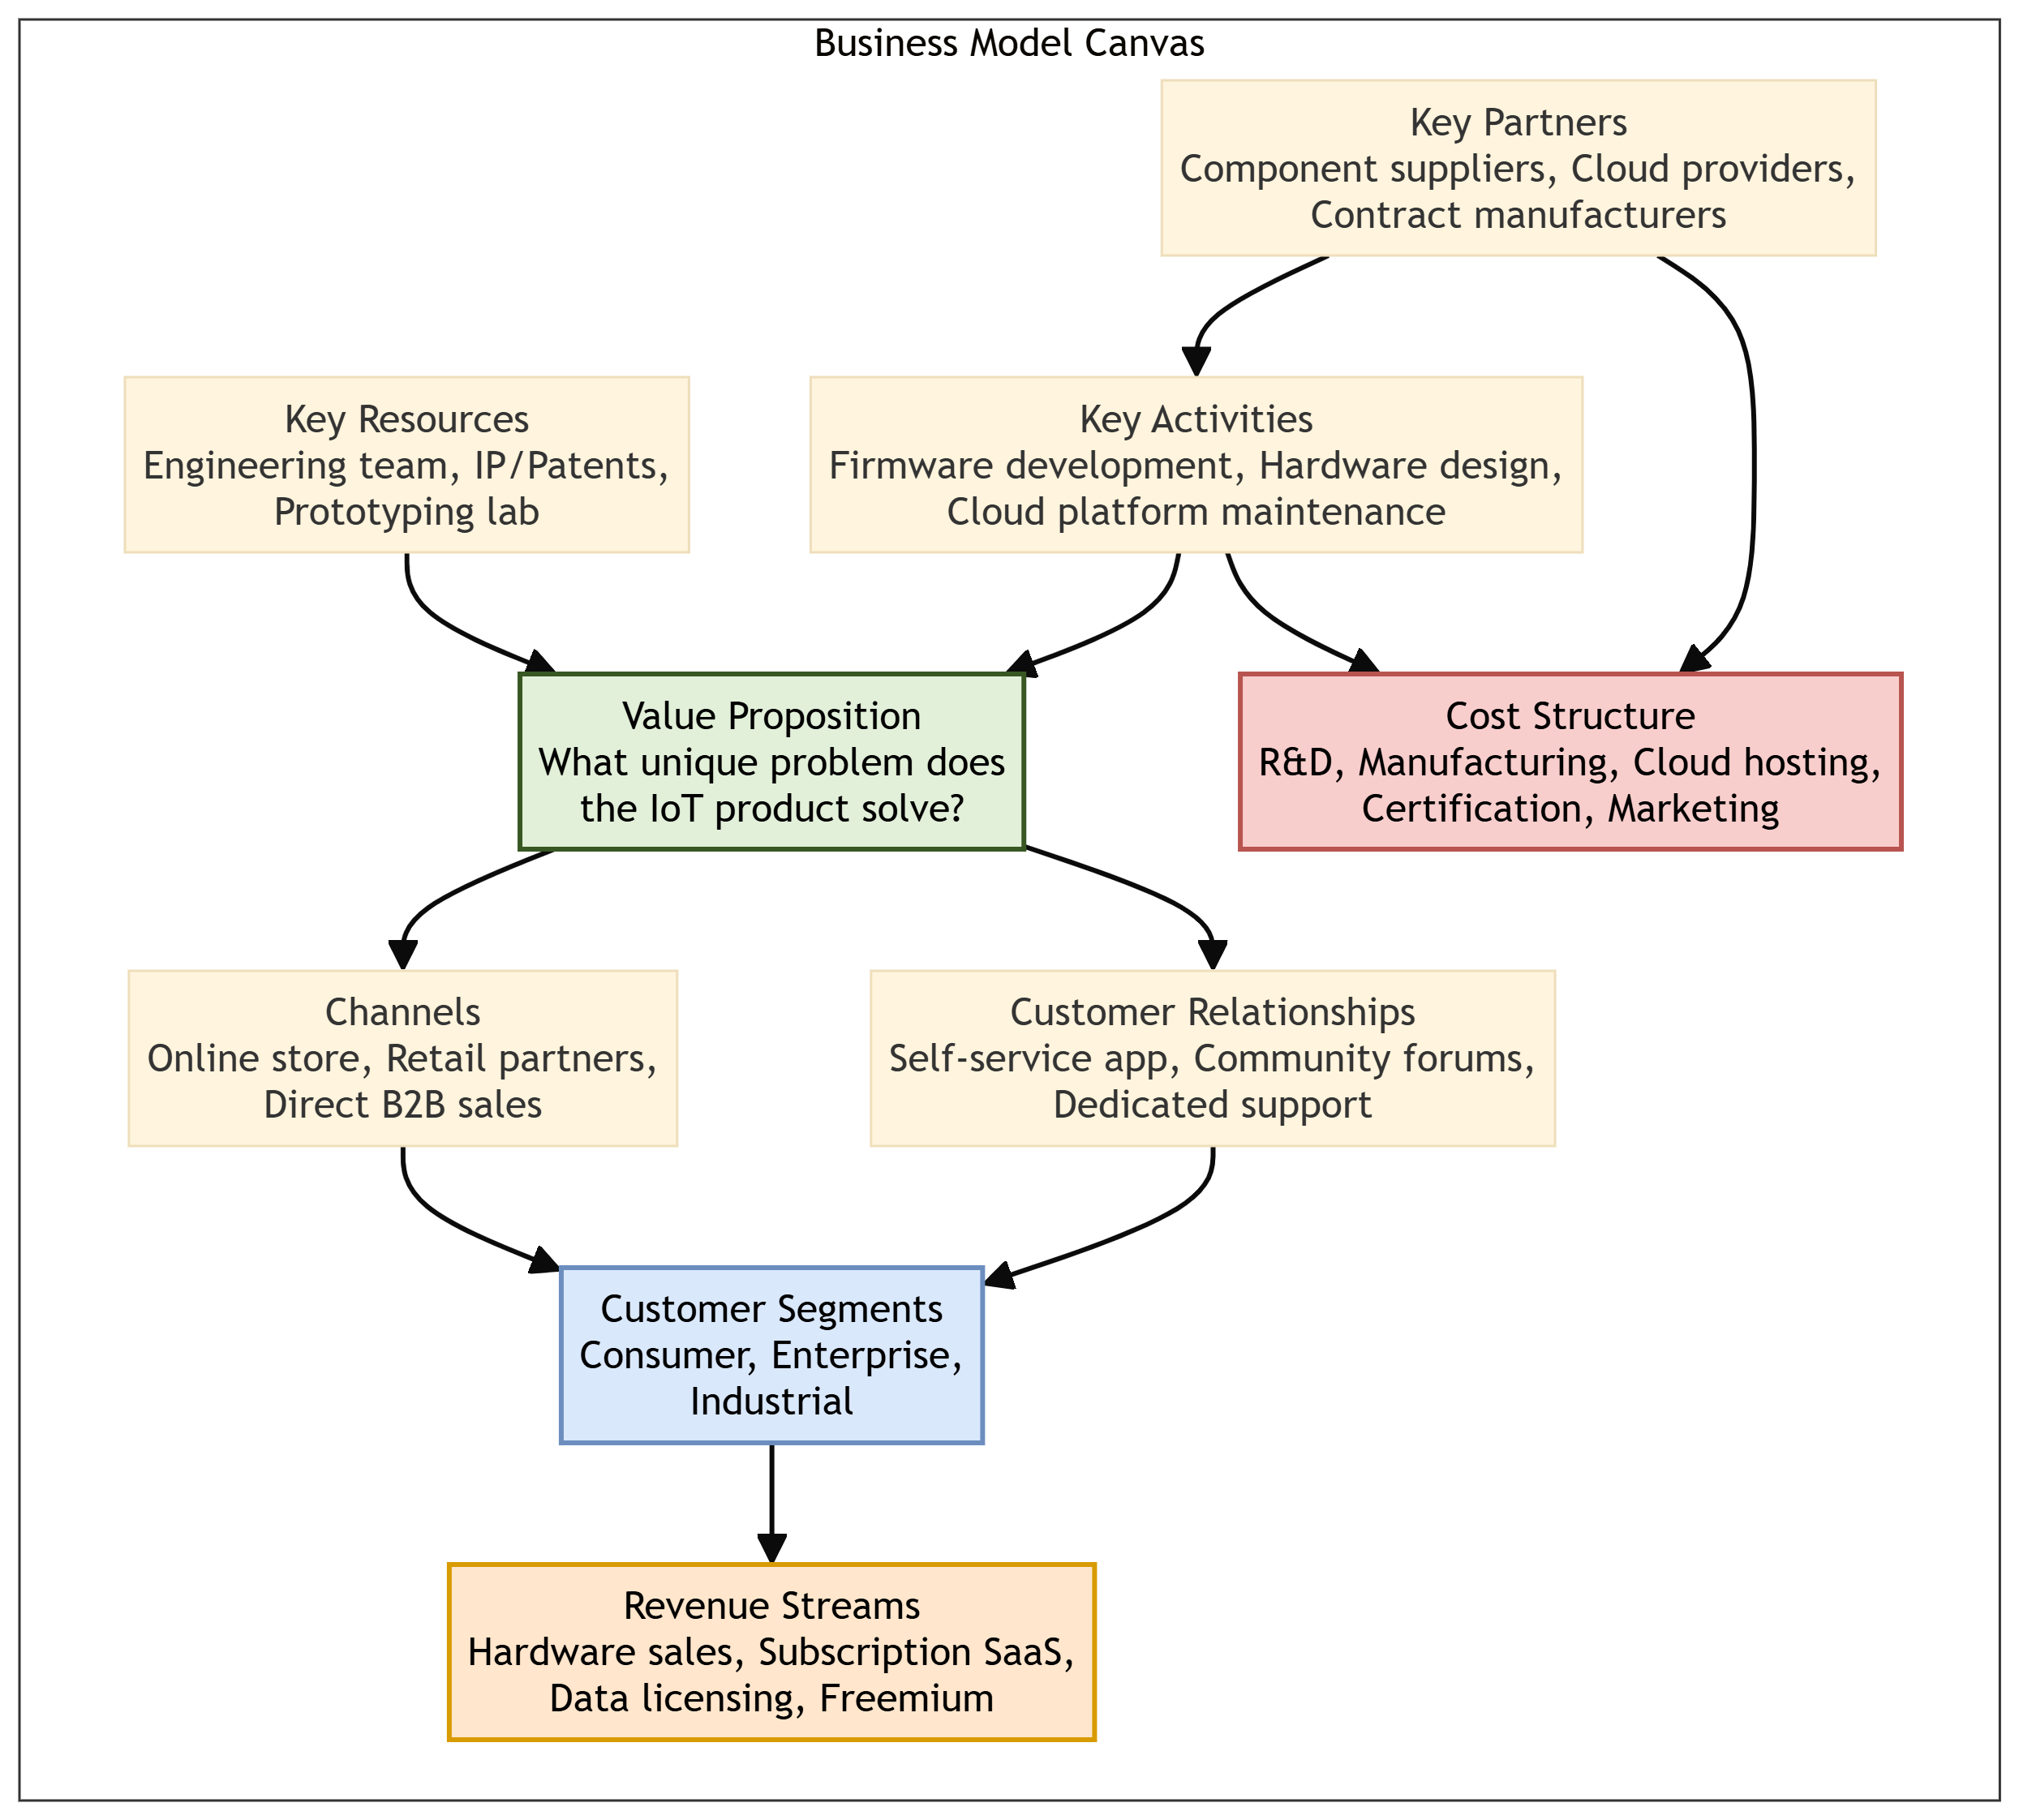
\includegraphics[width=0.75\textwidth,height=0.32\textheight,keepaspectratio]{../Images/chapter_08/business_model_canvas.png}
\caption{Business Model Canvas for IoT}
\end{figure}


\subsection{2. The Nine Building Blocks (Applied to IoT)}

\begin{table}[H]
\centering
\begin{tabular}{|p{\dimexpr 0.2\textwidth - 2\tabcolsep - 1.5\arrayrulewidth\relax}|p{\dimexpr 0.4\textwidth - 2\tabcolsep - 1.5\arrayrulewidth\relax}|p{\dimexpr 0.4\textwidth - 2\tabcolsep - 1.5\arrayrulewidth\relax}|}
\hline
\# & Block & IoT Application \\
\hline
1 & \textbf{Customer Segments} & Who are the target users? (e.g., Smart Home consumers, Industrial plant managers, Healthcare providers). \\
\hline
2 & \textbf{Value Proposition} & What unique problem does the IoT product solve that existing solutions do not? (e.g., 50\% energy savings via predictive HVAC control). \\
\hline
3 & \textbf{Channels} & How does the product reach the customer? (e.g., Online D2C store, retail partnerships, B2B direct sales). \\
\hline
4 & \textbf{Customer Relationships} & How is the customer engaged? (e.g., Self-service mobile app, community forums, dedicated account managers). \\
\hline
5 & \textbf{Revenue Streams} & How does the business earn money? (e.g., One-time hardware sale, recurring SaaS subscription for cloud analytics, data licensing). \\
\hline
6 & \textbf{Key Resources} & What assets are required? (e.g., Embedded engineering team, IP/patents, prototyping lab, cloud infrastructure). \\
\hline
7 & \textbf{Key Activities} & What must the business do? (e.g., Firmware development, hardware design, cloud platform maintenance, customer support). \\
\hline
8 & \textbf{Key Partnerships} & Who are the essential external partners? (e.g., Component suppliers, contract manufacturers, cloud platform providers like AWS/Azure). \\
\hline
9 & \textbf{Cost Structure} & What are the major costs? (e.g., R\&D salaries, BOM/component costs, cloud hosting, FCC/CE certification, marketing). \\
\hline
\end{tabular}
\end{table}


\subsection{3. Lean Startup Principles in IoT}

The \textbf{Lean Startup} methodology (Eric Ries) guides IoT ventures to minimize waste and maximize learning speed:

\subsubsection{A. Build-Measure-Learn Loop}
\begin{enumerate}
  \item \textbf{Build:} Create a \textbf{Minimum Viable Product (MVP)} — the simplest functional version of the IoT device (e.g., a breadboard prototype with a single sensor and a basic cloud dashboard).
  \item \textbf{Measure:} Deploy the MVP to a small group of early adopters. Collect quantitative data (e.g., usage frequency, feature engagement, error rates).
  \item \textbf{Learn:} Analyze the data. Determine whether the core hypothesis is validated (proceed) or invalidated (pivot — change the product direction).
\end{enumerate}

\subsubsection{B. Pivot or Persevere}
\begin{itemize}
  \item   After each Build-Measure-Learn cycle, the startup must decide:
  \item   \textbf{Persevere:} The data validates the hypothesis. Continue investing in the current product direction.
  \item   \textbf{Pivot:} The data invalidates the hypothesis. Change the customer segment, value proposition, or technology platform.
  \item   IoT pivots are common: a product designed for consumer smart home use may pivot to industrial monitoring if consumer adoption is low but factory interest is high.
\end{itemize}

\subsubsection{C. Validated Learning}
\begin{itemize}
  \item   Every experiment should produce \textbf{validated learning} — concrete, data-backed evidence about what customers actually want, not assumptions about what they should want.
\end{itemize}


\subsection{4. Advantages and Disadvantages of Lean Startup in IoT}

\subsubsection{Advantages:}
\begin{enumerate}
  \item Reduces financial risk by testing core assumptions before committing to expensive mass production tooling.
  \item Accelerates time-to-market by focusing only on features that customers actually use.
  \item Data-driven decisions replace guesswork.
\end{enumerate}

\subsubsection{Disadvantages:}
\begin{enumerate}
  \item Hardware MVPs are more expensive and slower to iterate than software MVPs (you cannot simply push a code update to fix a PCB design flaw).
  \item Early adopters may not represent the broader market, leading to biased validation.
  \item Constant pivoting can demoralize the engineering team and confuse early customers.
\end{enumerate}
